\documentclass[11pt]{article}

\usepackage{amsmath}    % need for subequations
\usepackage[utf8]{inputenc}
\usepackage{graphicx}   % need for figures
\usepackage{verbatim}   % useful for program listings
\usepackage{color}      % use if color is used in text
\usepackage{subfigure}  % use for side-by-side figures
\usepackage{hyperref}   % use for hypertext links, including those to external documents and URLs
\usepackage{afterpage}  % create blank page
\usepackage{appendix}   % create appendix
\usepackage[a4paper, margin=2cm]{geometry} % change margins
% \usepackage[french]{babel} % permet guillemets etc
\usepackage[british,UKenglish,USenglish,english,american]{babel}
\usepackage{wrapfig}
\usepackage{sectsty} % color title
\usepackage{eurosym}
\usepackage{tabularx}
\usepackage{anyfontsize}
\usepackage{tikz}
\usepackage{fancyhdr}
\usepackage{eso-pic}
\usepackage{minitoc}

%%%% Couleur des titres
\definecolor{green}{RGB}{134,188,37}
\definecolor{blue}{RGB}{98,181,229}
\definecolor{teal}{RGB}{0,151,169}

%%%% Themes
\fancypagestyle{theme}{
\fancyhf{}
\fancyhead[L]{}\fancyhead[C]{}\fancyhead[R]{\rightmark}
\fancyfoot[L]{Cassiopée 2018-2019}\fancyfoot[C]{\thepage}\fancyfoot[R]{}
\renewcommand*\headrulewidth{1pt}
\renewcommand{\footrulewidth}{1pt}
}

%%% Box
\newcommand{\titlebox}[2]{%
\tikzstyle{titlebox}=[rectangle,inner sep=10pt,inner ysep=10pt,draw]%
\tikzstyle{title}=[fill=white]%
%
\bigskip\noindent\begin{tikzpicture}
\node[titlebox] (box){%
    \begin{minipage}{0.94\textwidth}
#2
    \end{minipage}
};
%\draw (box.north west)--(box.north east);
\node[title] at (box.north) {#1};
\end{tikzpicture}\bigskip%
}

%% Custom packages
\usepackage{listings}

%%% Table
\usepackage{array,booktabs}
\usepackage{tabularx}
\usepackage{ragged2e}
\usepackage{hhline}
\newcolumntype{x}[1]
{>{\raggedright}p{#1}}
\newcolumntype{z}[1]
{>{\centering}p{#1}}
\newcommand{\tn}{\tabularnewline}
\renewcommand\tabularxcolumn[1]{>{\Centering}m{#1}}  

%%% Custom
\newcommand{\ptitle}[1]{\underline{\textsc{#1}} }
\newcommand{\Q}{\underline{\textsc{Question :}} }

\pagestyle{theme}

\thispagestyle{theme}

\newcolumntype{b}{X}
\newcolumntype{s}{>{\hsize=.5\hsize}X}
\usepackage{graphicx,lipsum}
\begin{document}

\begin{center}


\includegraphics[width=0.40\textwidth]{images/logo.png}  
\includegraphics[width=0.39\textwidth]{images/hackademint.png} \\ \vspace{2.5cm}

{\huge \textsc{Cassiopée Project 2018-2019: Development and deployment of an automated IT security audit tool in a virtualized environment.}} \\
  \textit{Aurélien Duboc, Pierrick Gorisse, Lucas Martin \\ Supervisor: Hervé Debar}

\end{center}

\vspace{2cm}
\begin{center}

\includegraphics[width=0.40\textwidth]{images/cassiopee.jpg}
\end{center}

\pagebreak

\noindent\rule{\textwidth}{.1pt}%
\tableofcontents
\noindent\rule{\textwidth}{.1pt}%

\pagebreak

\listoffigures

\pagebreak

% \section{Cassiopée Project: Development and deployment of an automated IT security audit tool in a
% virtualized environment.}
\section{Start of the project}


Large companies, as well as SMEs are subject to a security obligation
for their information systems. Our project proposes a tool that allows the
management of the main vulnerabilities that security auditers usually look for.
This tool identifies weaknesses and / or configuration vulnerabilities.
\\
The main interest lies in the automated analysis of a large number of machines.
It could also propose automated corrections associated with these weaknesses.
Our solution could be equivalent to a security audit for a company.

\vspace{1cm}
\subsection{Objectives}
\vspace{0.5cm}

\subsubsection{Infrastructure}

In order to provide a realistic framework for the implementation of such a tool, it is necessary to establish an active infrastructure resulting from the use of network services such as Virtual Private Networks (VPN), Domain Name Servers (DNS), reverse proxy, monitoring servers... It is also resulting from the use of personal services and data, as some users of this infrastructure host web and ftp servers on it.

\vspace{0.5cm}
\subsubsection{Setting up a security scan tools}

Our project focuses on developping a security audit tool for systems running UNIX environment, such as Linux or MacOS.
Windows security audit is an optional feature that is a project-building perspective.

\vspace{0.5cm}
\subsubsection{Management of the logs}
The management of the logs associated with these audits helps detect evidence of an attack in the logs of network devices, servers, and applications. The web interface aggregates and manages log data from built-in detection capabilities and from logs produced by other devices in your environment. It automatically executes advanced analysis, producing normalized events and correlating them to produce actionable intelligence, alerting us of any threats to the environment.


\vspace{0.5cm}
\subsubsection{Web interface}
The development of a web interface allowing data management and visibility over the data produced
by the log management tool.


\vspace{0.5cm}
\subsubsection{Build an opensource project}

Particpating in the development of this opensource tool requires competences such as mastering UNIX-like platforms (Linux, MacOS),
and associated tools (editors, interpretors, etc.).
%It works on a
%server without a graphical environment so a text editor like VIM should be
%Moptimized as an IDE with some plugins in order to increase the efficiency on the
%server side, on the development and deployment of the tool.
Coding in JavaScript and / or scripting languages, including referenced
frameworks for JavaScript development (e.g.~Node.js, Angular.js, etc.) might be usefull.
As Elasticsearch and Kibana are working as APIs, and frontend development part works
as a REST API (Representational State Transfer), REST standards have to be mastered as well in order to contribute on this project.

\pagebreak

\vspace{0.5cm}
\subsubsection{Learning objectives}
Processing of accessible textual data (coherence management, etc.)
, the presentation and analysis of textual data as well as the understanding of cybersecurity
software and integration. \\



\vspace{0.5cm}
\subsubsection{Documentation}
The use of English for our project is essential. Indeed, all the technical
documentation associated with the resources used is in English and we are used
to working with resources in English because they are much more complete. In
addition, the community providing these resources exchanges mainly in English. In order
to offer a tool that is widespread and easy to use, writing the
documentation in English then appears as a better choice. \\


\pagebreak

\subsection{Technical solutions}

\vspace{1cm}
\subsubsection{Setting up a hypervisor for managing virtualized content}

The chosen solution is Proxmox, an open source hypervisor that can provide container based virtual environment, using OpenVZ.
It supports guest operating systems like Linux (KVM), Windows. It is enabled by the presence of integrated backup service.
It delivers full system virtualization by the use of KVM.
The Proxmox management interface can function using a normal browser.
Proxmox is using the cluster mode: from a single page multiple servers can be managed.
It can also perform a direct migration from one host to another.
Lastly, Proxmox provides shell access to the KVM directly from its interface, using a Debian system.

\begin{figure}[!h]
  \centering
  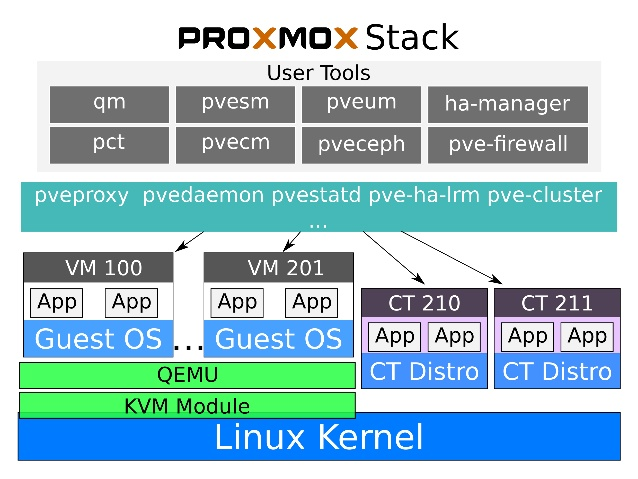
\includegraphics[width=0.6\textwidth]{images/proxmox-stack-example.jpg}
  \caption{Proxmox stack architecture}
  \label{Proxmox}
\end{figure}

\vspace{1cm}
Proxmox VE tightly integrates KVM (Kernel-based Virtual Machine) hypervisor and LXC
containers, software-defined storage and networking functionality on a
single platform, and easily manages high availability clusters and
disaster recovery tools with the built-in web management interface.

\vspace{0.5cm}
Qemu is running with the support of virtualization
processor extensions, via the Linux KVM module. In the context of
Proxmox VE, Qemu and KVM can be used interchangeably. Indeed, Qemu will always try to load the KVM module in Proxmox.

\\
\vspace{1cm}

*\url{https://www.proxmox.com/en/}

\pagebreak

\subsubsection{Setting up a directory to manage users and associated access control policies}

\vspace{0.4cm}

We use an LDAP directory [RFC 4510].
This allows a standardized representation of information (database - LDAP directory) as well as a standard query protocol widely deployed for this database.
The chosen solution is the OpenLDAP software version 2.4.46, because of its
maturity and protocol compliance. PhpLDAPadmin is the web interface that
allows the management of user accounts. One of the most important fields is
sshPublicKey because all the servers are configured to do LDAP queries
during an SSH connection to list the authorized RSA keys.
\\ We could have used a PAM setup with libpam-ldap but it seemed easier to specify
in ssh configuration files an AuthorizedKeyCommand that will reach all the
RSA public keys on the LDAP server.
\\
*\url{https://ldap.com/basic-ldap-concepts/}

\begin{figure}[!h]
  \centering
  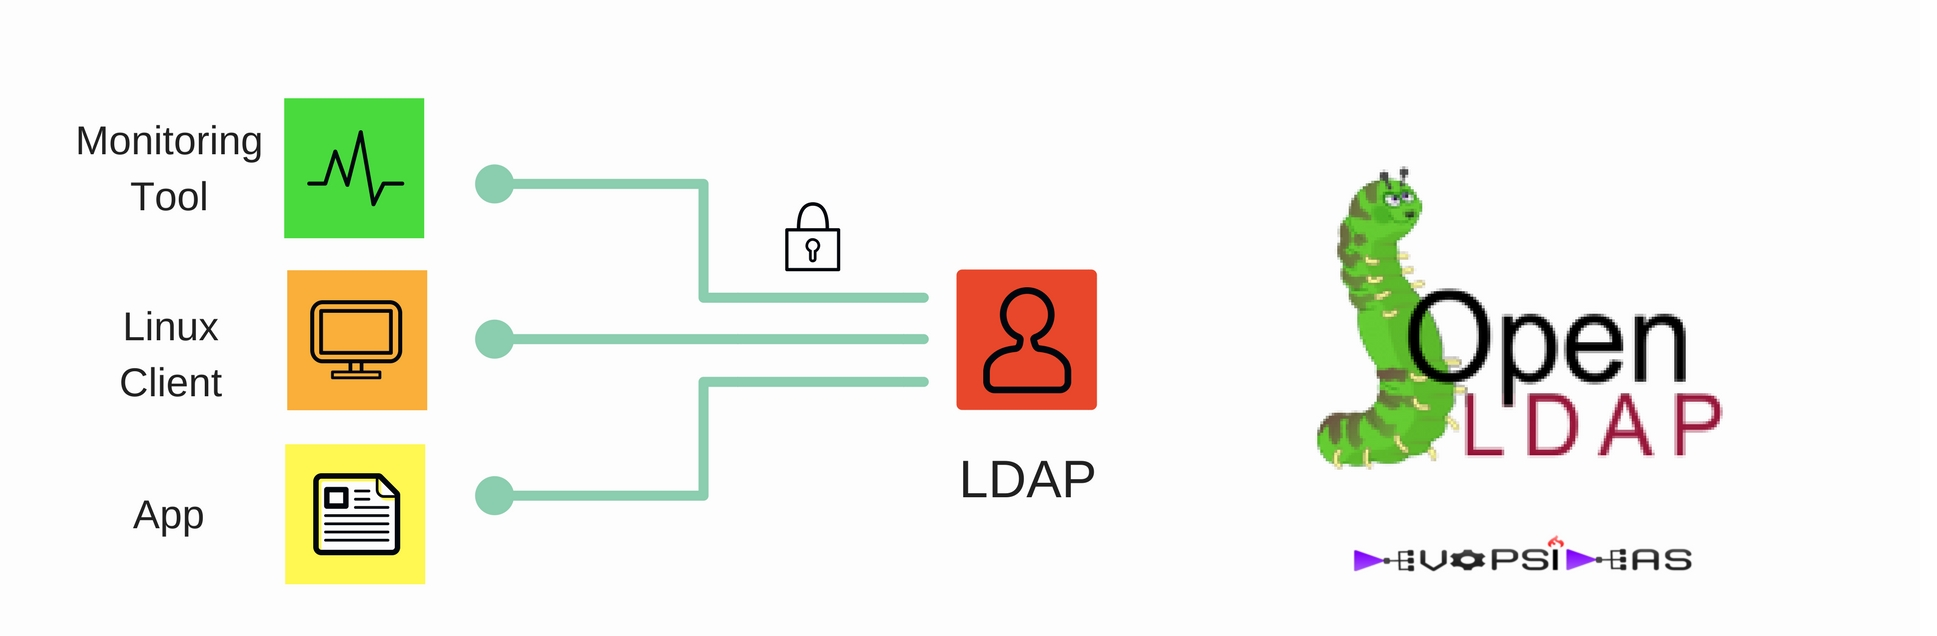
\includegraphics[width=0.75\textwidth]{images/ldap-example.png}
  \caption{Web Based LDAP Client}
  \label{LDAP}
\end{figure}

\subsubsection{Use of a tool allowing access to all virtualized machines while using the access control protocol cited above}
\vspace{0.5cm}

We chose Ansible, an open source software that automates software
provisioning, configuration management, and application deployment.
Ansible connects via SSH, remote PowerShell or via other remote APIs.\\ *
\url{(https://www.ansible.com/)}

\begin{figure}[!h]
  \centering
  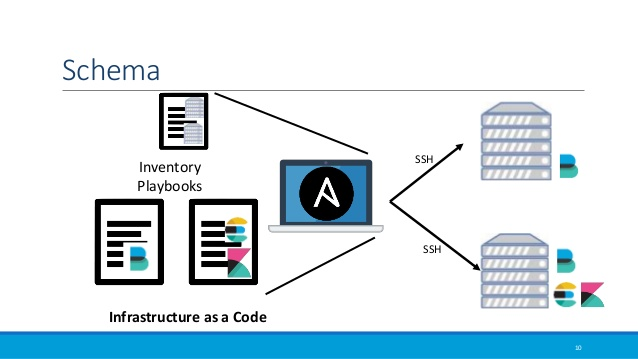
\includegraphics[width=0.75\textwidth]{images/ansible-example.jpg}
  \caption{Ansible playbooks deployment}
  \label{Ansible}
\end{figure}

\pagebreak

\subsubsection{Implementation of a list of tools allowing the automated audits added to our
  personal contribution}

For now, Lynis is the best candidate. We will probably combine several tools later.
Lynis is an extensible security audit tool for computer systems
running Linux, FreeBSD, macOS, OpenBSD, Solaris, and other
Unix-derivatives.
\\

Lynis scanning is opportunistic, meaning it will only use what it can find, like available tools or libraries. The benefit is that no installation of other tools is needed, so you can keep your systems clean.
By using this scanning method, the tool can run with almost no dependencies. Also, the more it finds, the more extensive the audit will be. In other words: Lynis will always perform scans that are customized to your system and two audits will never be the same.
\\

Many vulnerability scanners perform on a network level (outside of the system). They can detect missing security patches due to discovered weaknesses. However, in many cases leaks can be present, and their detection via the network close to impossible. An additional downside is version banners on which some of the tools rely, providing you with a false positive when the software vendor is using a patched version.
\\

Lynis focuses on scanning from the inside, on the system itself. This doesn’t mean it has to be installed on the system though. Lynis can run from local or external storage and only requires root permissions. The big benefit from running it on the system itself is that all information is available, including running processes, open network ports, being able to discover user accounts etc. Depending on your needs and how in-depth a security scan has to be, scanning from the inside might be a preferred method. More information will be available, while the chance of getting false positives is lower as well.

%\vspace{0.2cm}
%* \url{(https://cisofy.com/lynis/)}
\begin{figure}[!h]
  \centering
  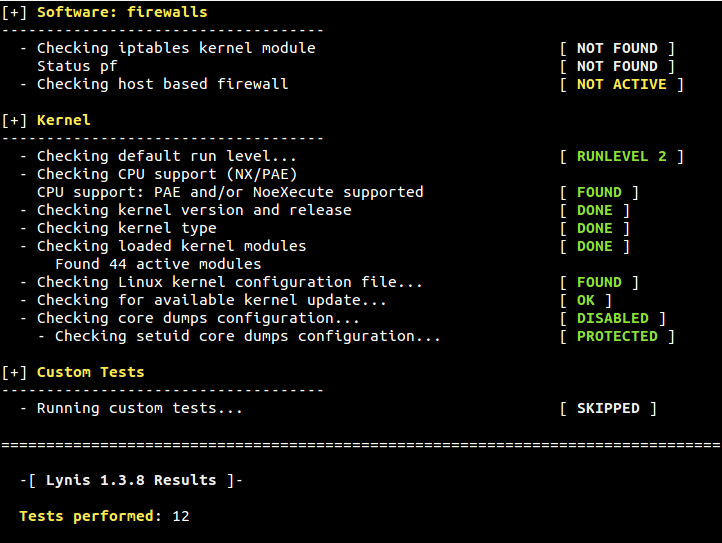
\includegraphics[width=0.95\textwidth]{images/lynis-example.png}
  \caption{Output from Lynis scan}
  \label{Lynis}
\end{figure}

\pagebreak

\subsubsection{Management of the logs}

ELK is the most famous tool for log processing and analysis, so naturally we will use this tool to generate our logs.
ELK is the acronym for three open source projects:
Elasticsearch, Logstash, and Kibana. Elasticsearch is a search and
analytics engine. Logstash is a server‑side data processing pipeline
that ingests data from multiple sources simultaneously, transforms it,
and then sends it to a stash like Elasticsearch. Kibana lets
users visualize data with charts and graphs in Elasticsearch.\\ *
\url{(https://www.elastic.co/fr/elk-stack)}\\


\begin{figure}[!h]
  \centering
  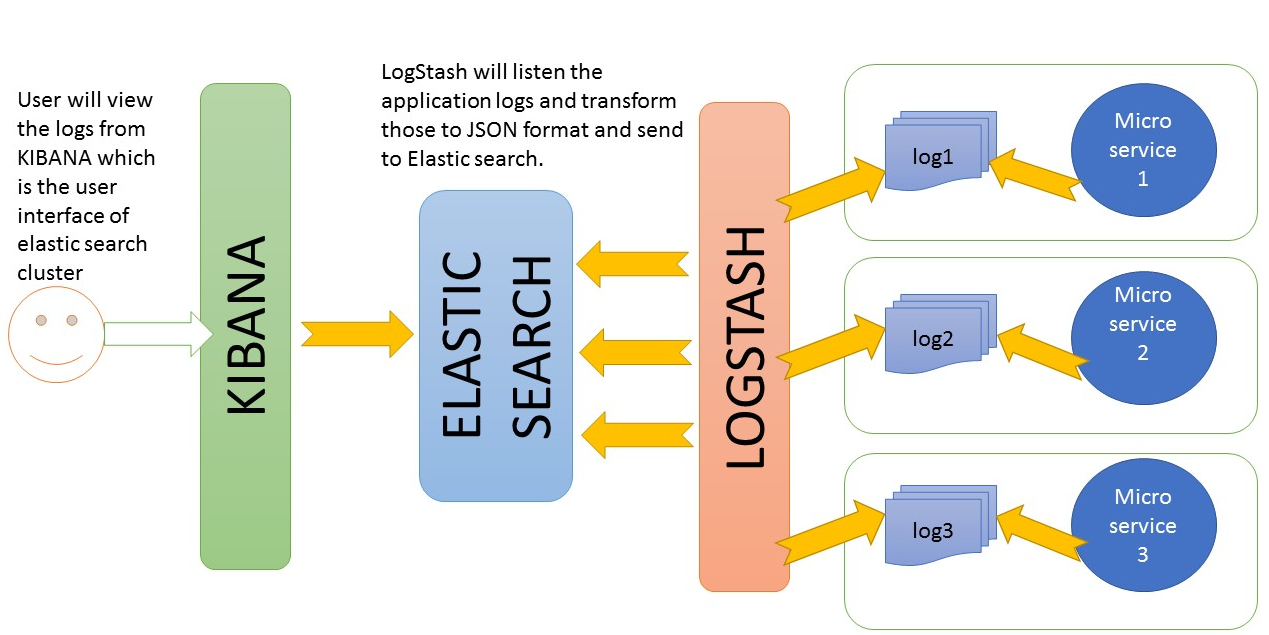
\includegraphics[width=0.75\textwidth]{images/elk-example.png}
  \caption{ELK stack interaction with different applications based on Log file}
  \label{ELK}
\end{figure}

\subsubsection{Web interface development}

The use of a framework associated with a certain number of libraries will
allow us to obtain a modular and easy to use application.
Symfony is a PHP framework that we used to work with, which is why we chose
to use this one. Moreover, we were able to verify that there were many
libraries usable in this framework that would allow us to interface ELK with our web
application. \\ *
\url{(https://pehapkari.cz/blog/2017/10/22/connecting-monolog-with-ELK/)}\\

\begin{figure}[!h]
  \centering
  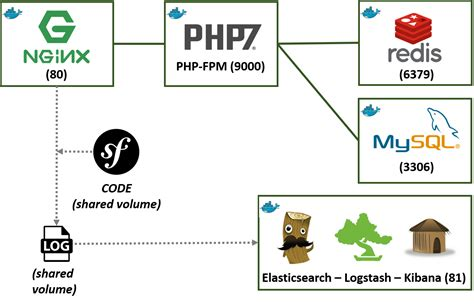
\includegraphics[width=0.65\textwidth]{images/symfony-example.jpg}
  \caption{First web application architecture}
  \label{Symfony}
\end{figure}

\pagebreak

\section{Implementation of the project}

\subsection{Update on the web development framework}

We finally chose to use Flask framework instead of Symfony, after further study of the following necessary features:
\begin{itemize}
    \item Elegant syntax, clear namespaces (providing good code-maintainability in the long term).
    \item Rich ecosystem and libraries (sqlalchemy, numpy, scipy, matplotlib).
    \item Out of box support for everything (such as large floating point numbers).
    \item Package management using pip is a breeze.
\end{itemize}

The use of Proxmoxer (\url{https://github.com/swayf/proxmoxer}) is also one of the main reasons for switching to a Python framework.
\\

Proxmoxer is a wrapper around the Proxmox REST API v2.
It was inspired by slumber, but it is dedicated only to Proxmox. It allows to use not only REST API over HTTPS, but the same API over ssh and pvesh utility as well.
Like Proxmoxia it dynamically creates attributes which responds to the attributes you've attempted to reach.

\begin{figure}[!h]
  \centering
  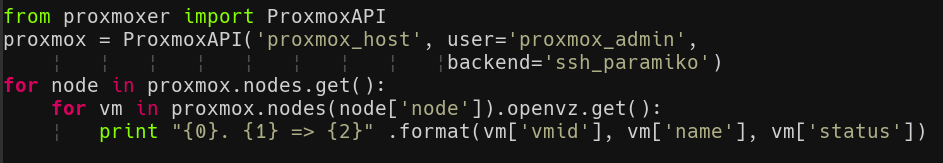
\includegraphics[width=0.99\textwidth]{images/proxmoxer.png}
  \caption{Snippet to get LXC and Qemu data over Proxmox API}
  \label{Proxmoxer}
\end{figure}

\pagebreak

\subsection{Network Architecture}

\vspace{2cm}

\begin{figure}[!h]
  \centering
  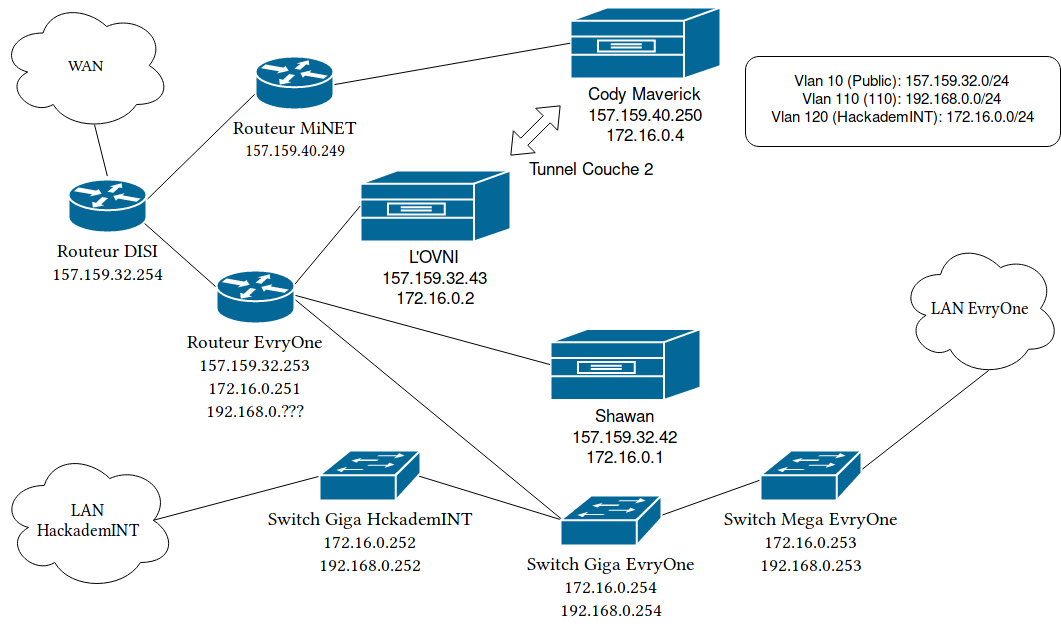
\includegraphics[width=0.95\textwidth]{images/reseau.png}
  \caption{Schema of the network architecture}
  \label{Proxmoxer}
\end{figure}

Three physical servers (whose names are "Cody-Maverick", "L'OVNI" and "Shawan") have been clustered on which are deployed the Proxmox hypervisor. These are DELL PowerEdge 1950 servers. The two Gigabit switches are Cisco SG500-52P 52-port Gigabit POE Stackable Managed Switch. The Megabit one is a Cisco Catalyst 3750.

\\
\vspace{1cm}

To connect to different machines in the infrastructure, the application
knows the IP addresses of the different machines, thanks to the API of
the hypervisor. RSA private keys must be inserted in the application by the system administrator to allow connection to
different machines.

\vspace{1cm}
\subsubsection{Technical specs of the servers}

The dual processor Dell PowerEdge 1950 delivers next generation performance in a 1U, rack dense chassis with Quad-Core Intel Xeon processors. This high concentration of computing power and redundancy makes the PowerEdge 1950 the perfect choice for high performance computing clusters (HPCC), SAN front-end, web and infrastructure applications. Outstanding manageability in this latest generation 1U server delivers new functionality for managing the servers from remote locations.

\pagebreak

\subsubsection{Virtual LANs}

A virtual LAN (VLAN) is any broadcast domain that is partitioned and isolated in a computer network at the data link layer (OSI layer 2). LAN is the abbreviation for local area network and in this context, virtual refers to a physical object recreated and altered by additional logic. VLANs work by applying tags to network frames and handling these tags in networking systems – creating the appearance and functionality of network traffic that is physically on a single network, but acts as if it is split between separate networks. In this way, VLANs can keep network applications separate despite being connected to the same physical network, without requiring multiple sets of cabling and networking devices to be deployed.

\\
\vspace{1cm}
The three clustered servers are separated by three routers and we do not have access to one of them, so we have established a network infrastructure in which we have installed VLANs while the subnets are schemas-filled. In order to realize the cluster between the servers, we set up an Ethernet layer 2 bridge (see next subsection).

\vspace{1cm}
\subsubsection{Layer 2 ethernet bridging}

Layer-2 bridging works by putting one physical and one virtual Ethernet adapter into a mode where they can receive traffic that is not destined to their address. This traffic is selectively sent onto the other network according to the IEEE 802.1D standard, known as "bridging" the frames. Frames transmitted by virtual Ethernet adapters on the same VLAN as the bridging virtual Ethernet adapter can be sent to the physical network. Frames sent from the physical network can be received by adapters on the virtual network.

\pagebreak

\subsection{Application Architecture}

Here is the detail of the architecture as currently designed for this project:
\vspace{1cm}

\begin{figure}[!h]
  \centering
  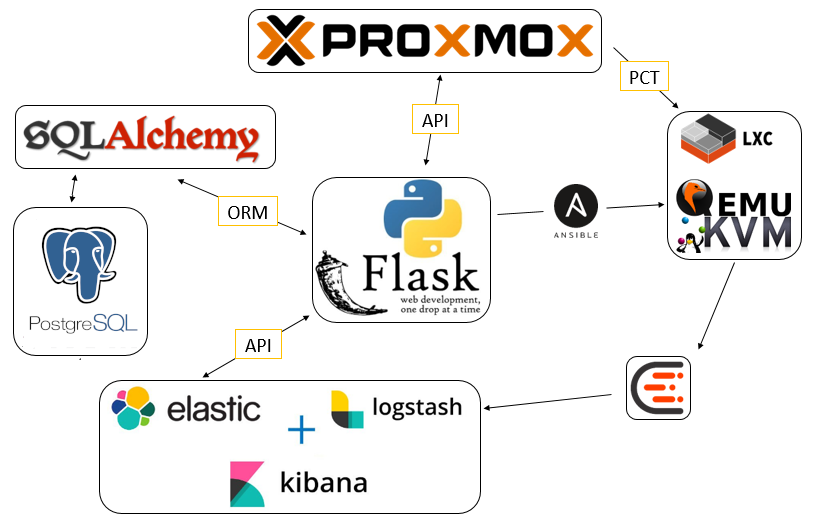
\includegraphics[width=0.90\textwidth]{images/schema.png}
  \caption{Application architecture schema}
  \label{ArchitectureSchema}
\end{figure}

\begin{itemize}
\item
  Flask application interacts with this hypervisor through its API. We
  so use proxmoxer as a wrapper to interface with
  it.
\item
  It is possible to access containers and virtual machines through
  pct (Tool to manage Linux Container (LXC) on Proxmox VE) and
  qmu (Qemu / KVM Virtual Machine Manager).
\item
  By using the SSH network protocol, the Ansible tool helps with the execution of
  Lynis security audit tool on the different containers. This generates a
  log file which will then be parsed in the ELK stack, itself
  interfaced with the application. We thus obtain a complete report of the
  security of every machine within the application.
\item
  User management of the application is performed at a base level
  postgresql data that the application accesses via the SQlachemy ORM.
\end{itemize}


\pagebreak

\subsection{Scoring and standardization}

\vspace{1cm}
\\
With Lynis, many tests are part of common security guidelines and standards,
completed with additional security tests. After the scan a report will be displayed
with all discovered vulnerabilities. Our application will map these vulnerabilities with a CVSS Base, Temporal and Enrironmental Score.

\vspace{0.2cm}

\begin{figure}[!h]
  \centering
  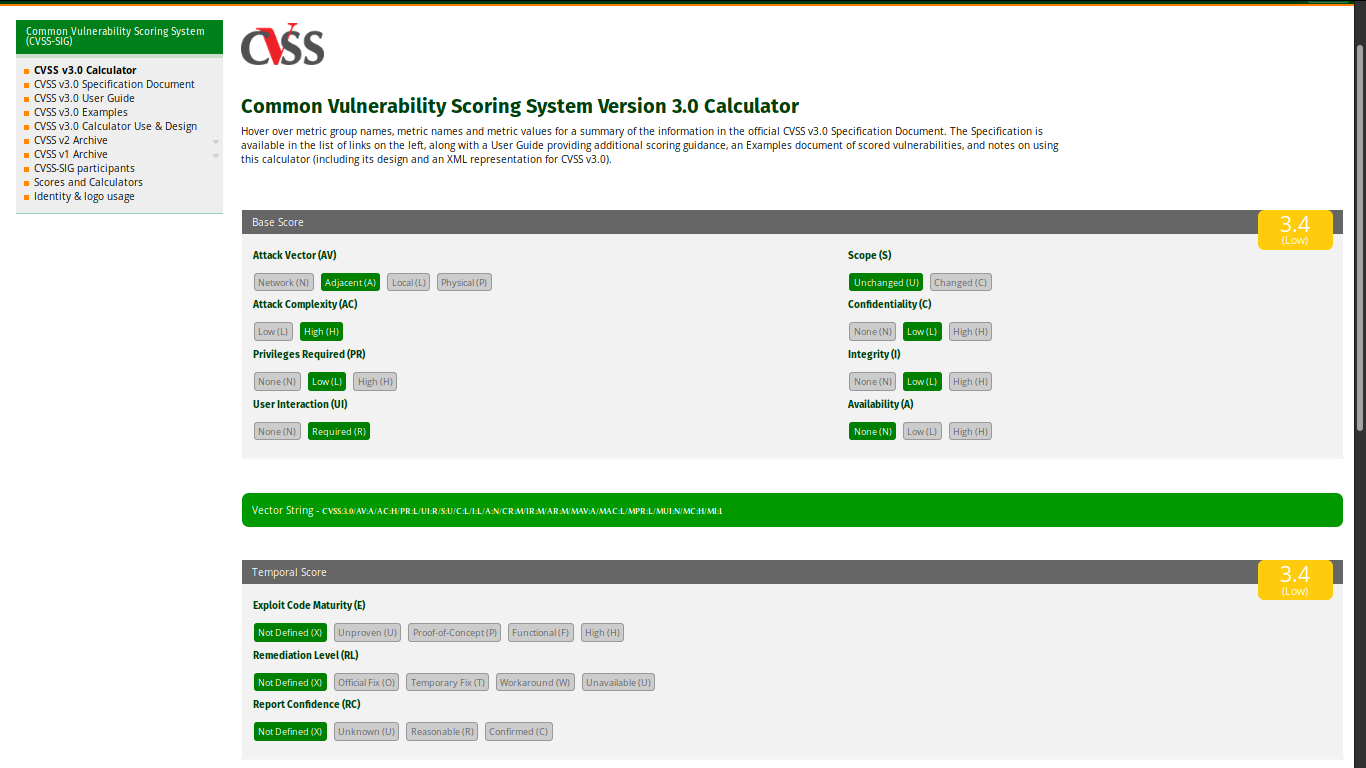
\includegraphics[width=0.98\textwidth]{images/cvss.png}
  \caption{Common Vulnerability Scoring System Version 3.0 Calculator}
  \label{ArchitectureSchema}
\end{figure}

\vspace{1cm}

\\
The Common Vulnerability Scoring System (CVSS) is a free and open industry standard for assessing the severity of computer system security vulnerabilities. CVSS attempts to assign severity scores to vulnerabilities, allowing responders to prioritize responses and resources according to threat. Scores are calculated based on a formula that depends on several metrics, that approximate ease of exploit and the impact of exploit. Scores range from 0 to 10, with 10 being the most severe. While many utilize only the CVSS Base score for determining severity, temporal and environmental scores also exist, to factor in availability of mitigations and how widespread vulnerable systems are within an organization, respectively.

\\
\vspace{0.2cm}
\url{https://www.first.org/cvss/calculator/3.0}

\pagebreak

\section{Results}

\subsection{Login View}
url: \url{https://cassiopee.hackademint.org/login}

\begin{figure}[!h]
  \centering
  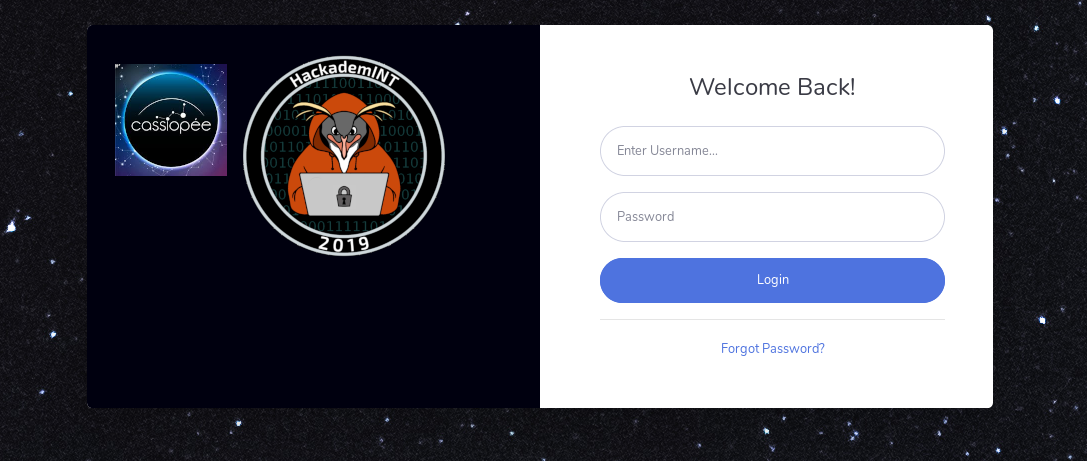
\includegraphics[width=0.98\textwidth]{images/flask-application-01.png}
  \caption{Screenshot of Login View}
  \label{LoginView}
\end{figure}


\subsection{Admin Panel}
url: \url{https://cassiopee.hackademint.org/admin/users/}

\begin{figure}[!h]
  \centering
  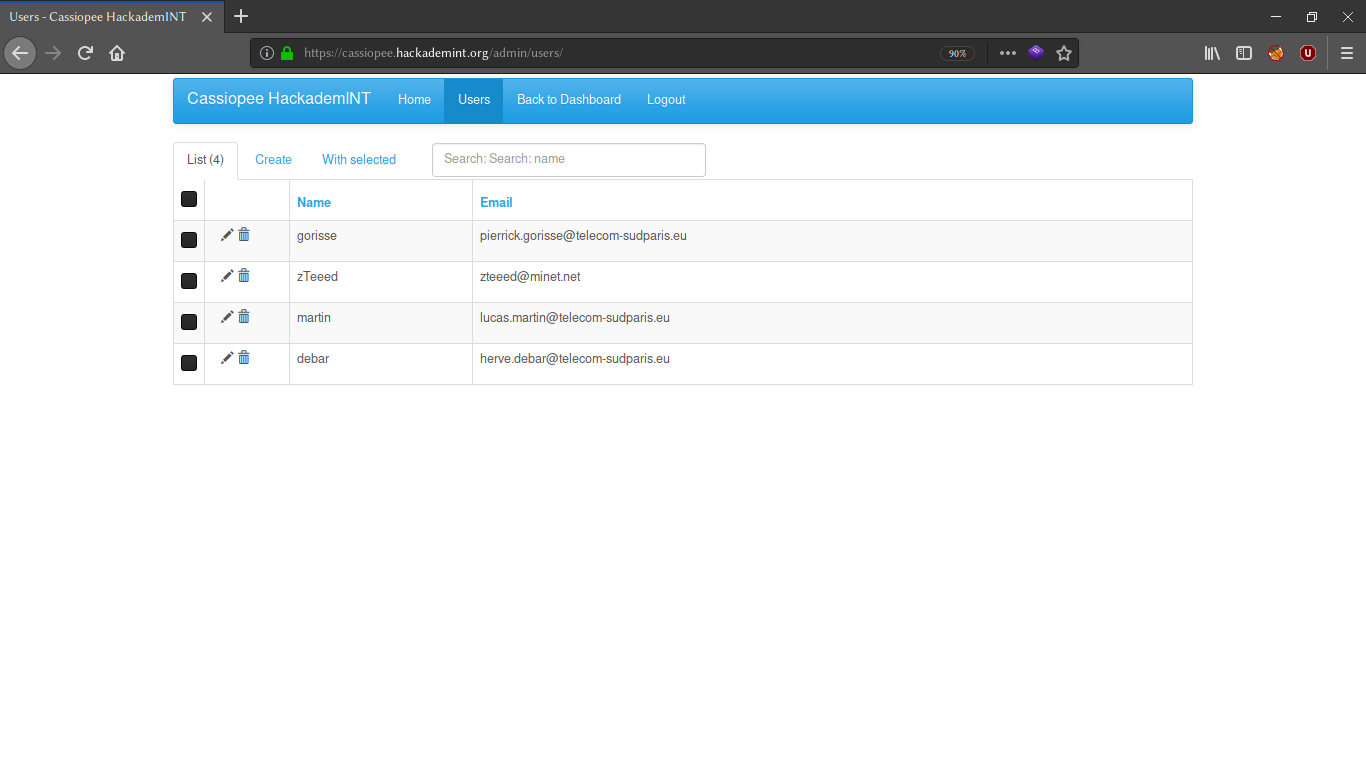
\includegraphics[width=0.88\textwidth]{images/flask-application-0.png}
  \caption{Screenshot of Admin Panel}
  \label{AdminPanel}
\end{figure}

This admin panel allows to manage the administrators of the platform

\pagebreak

\subsection{Forgot View}
url: \url{https://cassiopee.hackademint.org/forgot}

\begin{figure}[!h]
  \centering
  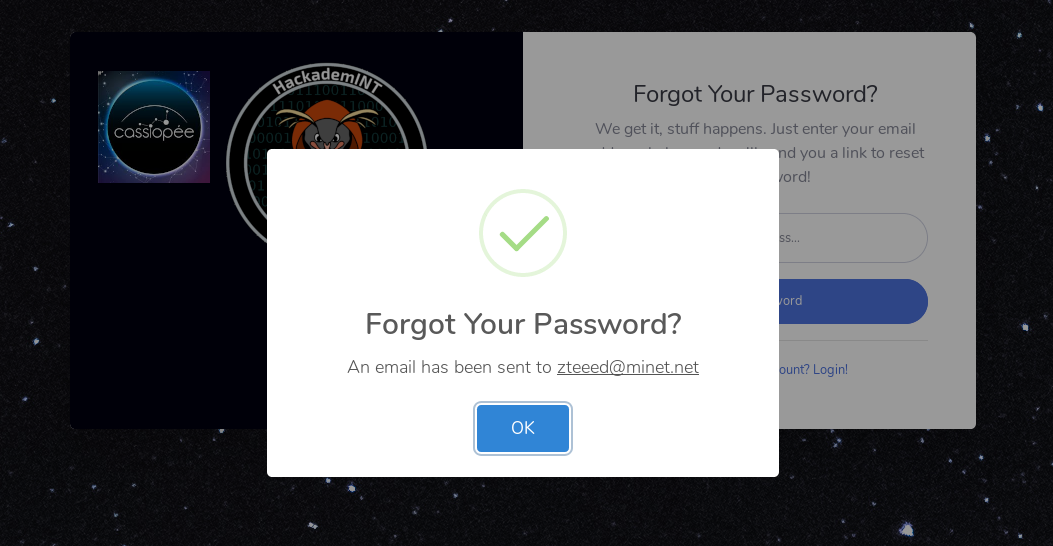
\includegraphics[width=0.98\textwidth]{images/flask-application-02.png}
  \caption{Screenshot of Forgot View}
  \label{ForgotView}
\end{figure}


\begin{figure}[!h]
  \centering
  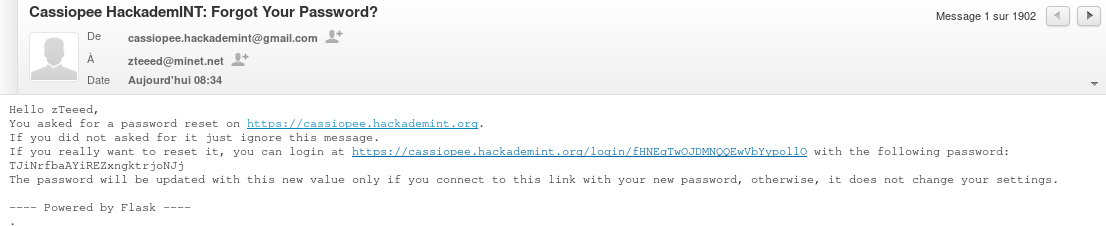
\includegraphics[width=1.05\textwidth]{images/flask-application-021.png}
  \caption{Screenshot of Email sent by Forgot View}
  \label{ForgotViewSent}
\end{figure}


\pagebreak

\subsection{Index View}

\begin{figure}[!h]
  \centering
  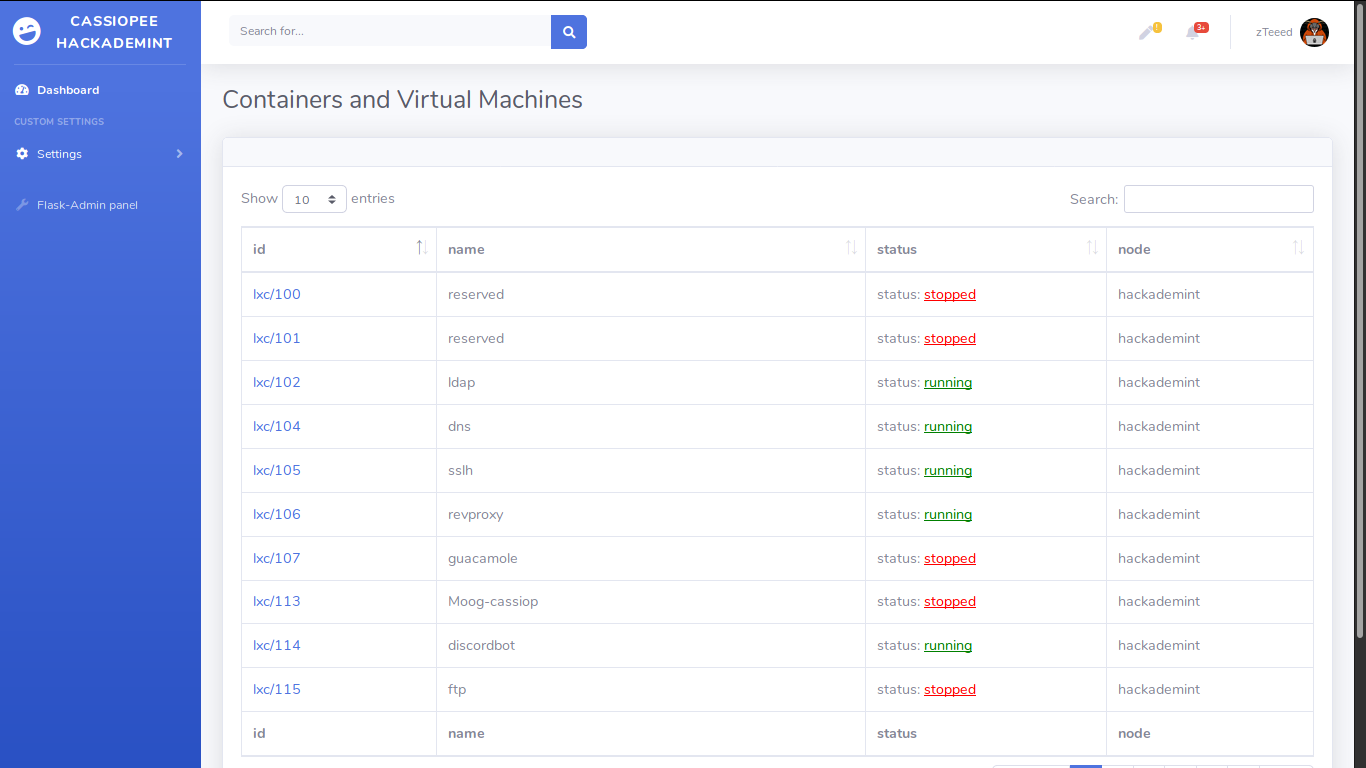
\includegraphics[width=1.05\textwidth]{images/flask-application-1.png}
  \caption{Screenshot of Index View}
  \label{IndexView}
\end{figure}

\pagebreak

\subsection{CT/VM view}

\begin{figure}[!h]
  \centering
  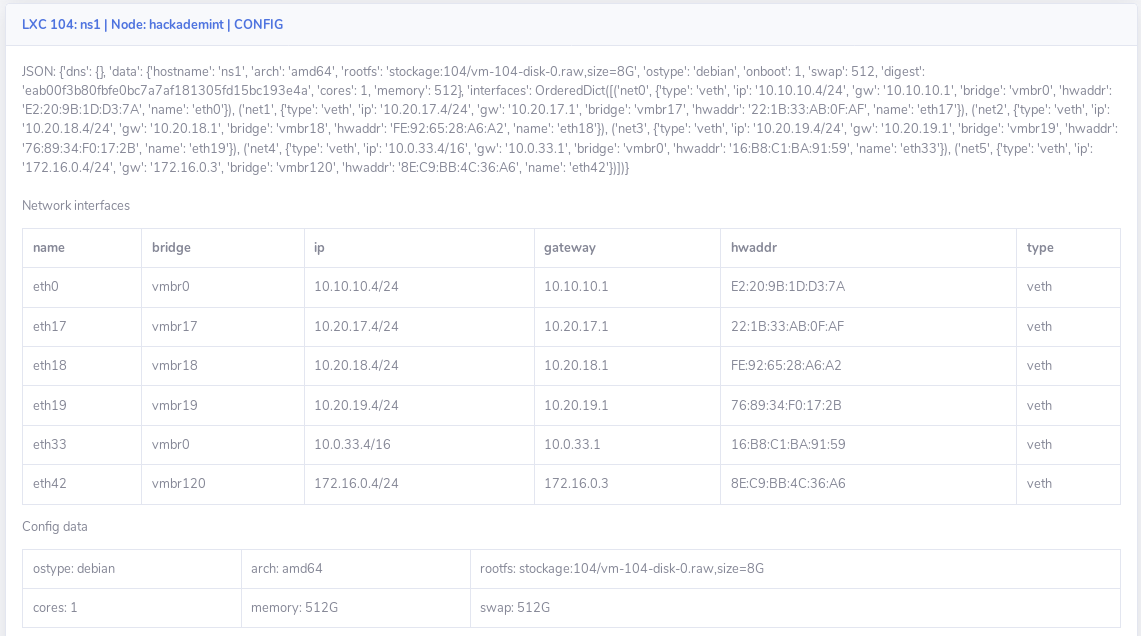
\includegraphics[width=1.05\textwidth]{images/flask-application-2.png}
  \caption{Screenshot of CT/VM View 1}
  \label{CTView}
\end{figure}

\begin{figure}[!h]
  \centering
  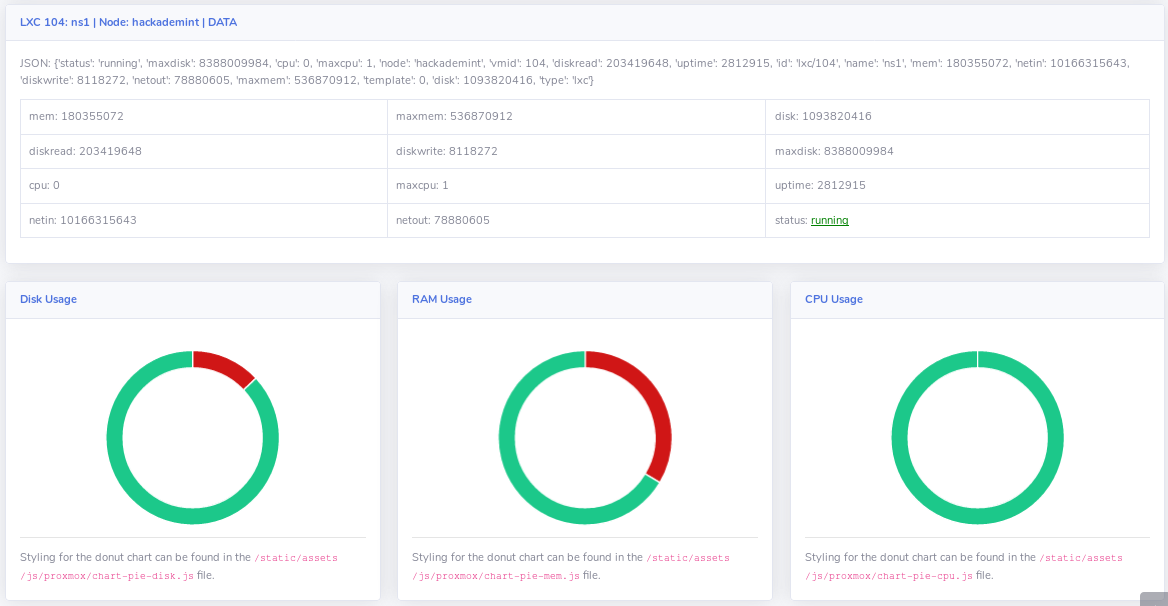
\includegraphics[width=1.05\textwidth]{images/flask-application-3.png}
  \caption{Screenshot of CT/VM View 2}
  \label{CTView2}
\end{figure}

\pagebreak

\begin{figure}[!h]
  \centering
  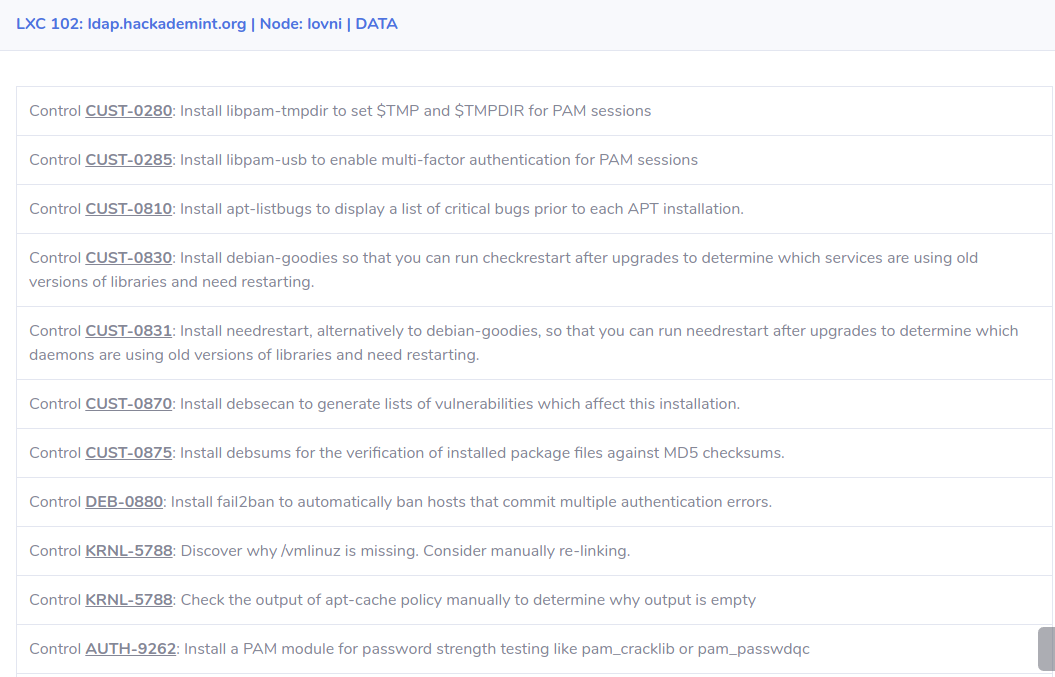
\includegraphics[width=1.05\textwidth]{images/flask-application-4.png}
  \caption{Screenshot of Security results}
  \label{CTView3}
\end{figure}

\pagebreak

\section{Conclusion and perspectives}


This project allowed us to provide an opensource tool for internal audit of a virtualized environment for system administrators.
Deployment with docker allows an easy deployment and quick and efficient tool handling

Some perspectives can be expected such as:
\begin{itemize}
  \item{Windows internal audit}
  \item{External audit}
  \item{The integration new tools for internal or external audit of the virtualized environment in addition to Lynis}
\end{itemize}


\end{document}
